% !TEX root =  MAIN.tex

\newpage
\subsection{Developed Toolset - SEMuS}
\label{sec:semus}

\STARTCHANGEDWPT

\TODO{This is the sentence in which you want to explain what is the solution implemented in FAQAS. You have to wrte something like "To achieve test suite augmentation (i.e., automatically generate test cases that kill mutants), in FAQAS, we have implemented an extension of SEMu that we call..."}

To achieve test suite augmentation (i.e., automatically generate test cases that kill mutants), in FAQAS, we have implemented an extension of SEMu that we call SEMu for Space Software (SEMuS).

%Symbolic Execution-based Mutant analysis for Space software (FAQAS-SEMuS), is an extension of SEMu that implements test generation for space software. 

\TODO{First you need to explain why SEMu cannot be used as in in FAQAS}

\begin{figure}[tb]
\begin{center}
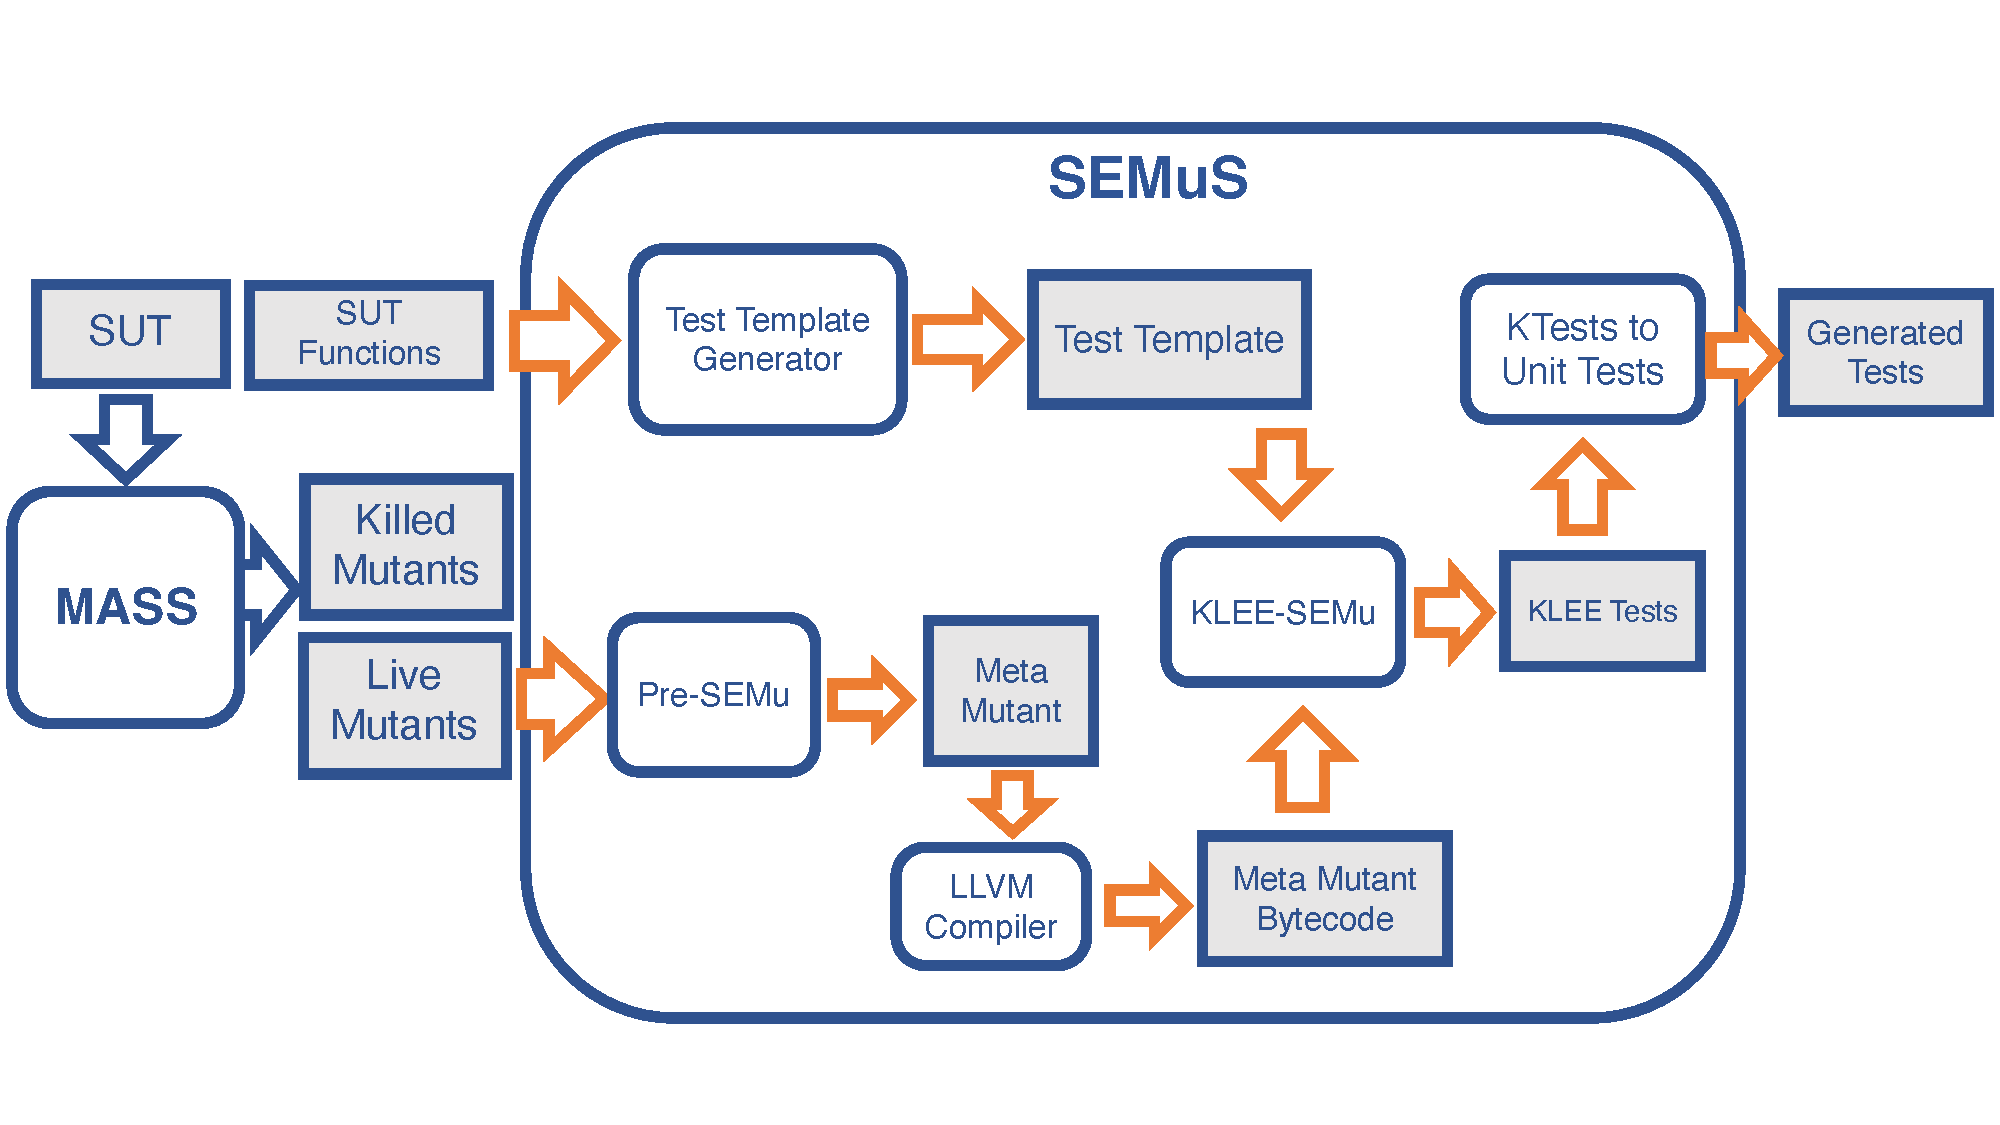
\includegraphics[width=0.8\textwidth]{images/semus-architecture}
\caption{FAQAS-SEMuS Architecture and Workflow}
\label{fig:semus_architecture}
\end{center}
\end{figure}

Figure~\ref{fig:semus_architecture} shows the architecture of SEMuS and how it interacts with MASS.

%SEMuS receives the following inputs: (a) the list of live mutants (produced by MASS), (b) the SUT, and (c) the SUT functions. 

As shown in Figure~\ref{fig:semus_architecture} SEMus is composed by five components, which are \emph{Test Template Generator},  \emph{Pre-SEMu},  \emph{KLEE-SEMu},  \emph{KTest to Unit Test}, and \emph{LLVM}.

\TODO{Why the following listing appears here? Can't we put it top or bottom?}
% !TEX root =  ../MAIN.tex

\begin{lstlisting}[style=CStyle, caption=SEMuS test template., label=test_template]
int main(int argc, char** argv) {
    // Declare variable to hold function returned value
    _Bool result_faqas_semu; 
    // Declare arguments and make input ones symbolic
    unsigned long pVal;
    int pErrCode;
    klee_make_symbolic(&pVal, sizeof(pVal), "pVal"); // Call function under test
    result_faqas_semu = T_INT_IsConstraintValid(&pVal, &pErrCode); // Make some output
    printf("FAQAS-SEMU-TEST_OUTPUT: %d\n", pErrCode);
    printf("FAQAS-SEMU-TEST_OUTPUT: %d\n", result_faqas_semu);
    return (int)result_faqas_semu;
}

\end{lstlisting}


\begin{lstlisting}[language={}, caption=Klee-test output, label=ktest]
ktest file : 'test000001.ktest'
args       : ['/MakeSym-TestGen-Input/direct/T_INT_IsConstraintValid/test.MetaMu.bc']
num objects: 2
object    0: name: b'model_version'
object    0: size: 4
object    0: data: b'\x01\x00\x00\x00'
object    1: name: b'pVal'
object    1: size: 8
object    1: data: b'\x00\x00\x00\x00\x00\x00\x00\x00'
\end{lstlisting}

\TODO{You need to provide the idea behind SEMus, that is, what it does at a high level. You need to say that the objective is to generate automatically a test template including symbolic variables and ...}

The \emph{Test Template Generator} (TTG) component automates the generation of templates for the symbolic execution search. The component receives as inputs the SUT source code and the list of SUT functions. 
Listing~\ref{test_template} shows an example of a test template generated by the TTG. The TTG generates a template for every SUT function; as shown in Listing~\ref{test_template} the component parses the function arguments and declares them symbolic through use of the KLEE function \texttt{klee\_make\_symbolic}. Then, it adds a call to the function under analysis with symbolic values, and it saves the output into the variable \texttt{result\_faqas\_semu}. Finally, the TTG adds a return call with the \texttt{result\_faqas\_semu} variable value.

The \emph{Pre-SEMu} component generates \INDEX{mutant schemata}; specifically, the component includes and compiles all the live mutants (i.e., MASS output) into a single bytecode file named the \emph{Meta Mutant}. At runtime, SEMu will select which mutant to consider for test generation based on a parameter. The compilation of the Meta Mutant into LLVM bitcode is supported by the \emph{LLVM} compiler infrastructure. 

\TODO{This listing should appear top or bottom, no?}
% !TEX root =  ../MAIN.tex
\begin{lstlisting}[float=t, language={}, caption=Klee-test output, label=ktest]
ktest file : 'test000001.ktest'
args       : ['/MakeSym-TestGen-Input/direct/T_INT_IsConstraintValid/test.MetaMu.bc']
num objects: 2
object    0: name: b'model_version'
object    0: size: 4
object    0: data: b'\x01\x00\x00\x00'
object    1: name: b'pVal'
object    1: size: 8
object    1: data: b'\x00\x00\x00\x00\x00\x00\x00\x00'
\end{lstlisting}

\emph{KLEE-SEMu} is the underlying test generation component, previously described in Section~\ref{klee-semu}. This component receives as inputs the \emph{LLVM bitcode Meta Mutant} and the \emph{Test Template} for the function under test, and proceeds to apply dynamic symbolic execution to generate test inputs to kill the mutants. The output of this component are the \emph{KLEE tests}.
\TODO{you need to list what are "the parameters of the execution"}
A KLEE test is a binary file that contains information about the execution of KLEE such as the entry point of the analysis, and the generated test inputs.

\TODO{I fixed the following. You always have first to describe the structure of the listing and then explain its content}
An example of a KLEE test is presented in Listing~\ref{ktest}. The field \emph{args} report the entry point of the analysis; in this case, the test generation was performed for live mutants present in the function \texttt{T\_INT\_IsConstraintValid}, which SEMuS stores in a dedicated folder. The fields named \emph{object} provide information about the outputs generated by KLEE (e.g., the generated test inputs). 
For each object, the KLEE test provides a \emph{name} (usually the name of the symbolic variable), its \emph{size}, and the actual \emph{value} generated by KLEE through constraint solving (usually this is reported in binary form).
Objects are numbered. Object number \emph{0} reports information about the data structure used by KLEE, that is, the version of the structure. The other objects report information about the generated test inputs.
Our example shows that one value of size 8 was generated for the variable \texttt{pVal}, the data field shows the binary representation of the \texttt{pVal} variable, in this case \texttt{pVal=0}.


% !TEX root =  ../MAIN.tex

\begin{lstlisting}[float=t, style=CStyle,  caption=Generated test case, label=gen_test_case]
#include <stdio.h>
#include <string.h>

#include "asn1crt.c"
#include "asn1crt_encoding.c"
#include "asn1crt_encoding_uper.c"


int main(int argc, char** argv)
{
    (void)argc;
    (void)argv;

    // Declare variable to hold function returned value
    _Bool result_faqas_semu;

    // Declare arguments and make input ones symbolic
    unsigned long pVal;
    int pErrCode;
    memset(&pVal, 0, sizeof(pVal));
    const unsigned char pVal_faqas_semu_test_data[] = {0x00, 0x00, 0x00, 0x00, 0x00, 0x00, 0x00, 0x00};
    memcpy(&pVal, pVal_faqas_semu_test_data, sizeof(pVal)); // Unsigned val is 0

    // Call function under test
    result_faqas_semu = T_INT_IsConstraintValid(&pVal, &pErrCode);

    // Make some output
    printf("FAQAS-SEMU-TEST_OUTPUT: pErrCode = %d\n", pErrCode);
    printf("FAQAS-SEMU-TEST_OUTPUT: result_faqas_semu = %d\n", result_faqas_semu);
    return (int)result_faqas_semu;
}
\end{lstlisting}

\TODO{I updated the following, please check}

The component \emph{KTest to Unit Test} (KTU)  converts a KLEE test into a readable, executable C test case. Similar to the TTG component, the KTU uses a template to hold the specifics variables of each function under test. 
Listing~\ref{gen_test_case} shows an example of a test case generated for a mutant present in the function \texttt{T\_INT\_IsConstraintValid}. For instance, line 20 shows that the variable \texttt{pVal} is initially filled with 0 (to clean it), then in line 21, it is filled with the value stored in the variable \texttt{pVal\_faqas\_semu\_test\_data}, which holds the binary output produced by KLEE. In line 25, the function under test is invoked with the concrete value of \texttt{pVal}. Finally, the KTU print the function return value and the value of every variable passed by reference.
At the current stage, KTU does not generate assertions. Assertions need to be implemented by engineers in place of the generated \emph{printfs} because only the engineers can know, based on specifications, what are the values to be expected at the end of the test case execution.


\ENDCHANGEDWPT
